\section{基于Zigzag映射矩阵的时间隐通道构建方法}
\label{chap:zigzag:model}

本节对构建方法进行详细介绍,包括设计架构、调制流程及解调流程三个部分。设计架构部分,主要介绍该时间隐通道的主要流程,引入的处理环节及处理对象变化情况。调制流程部分,主要介绍调制过程中的流程、计算方法及数据处理流程。解调流程部分,主要介绍解调过程中,如何根据丢包序号还原隐蔽消息,包括数据转换及数据检验等部分。

\subsection{设计架构}
\label{chap:zigzag:model:system}

\insertFigure{
	\begin{figure}
		\centering
        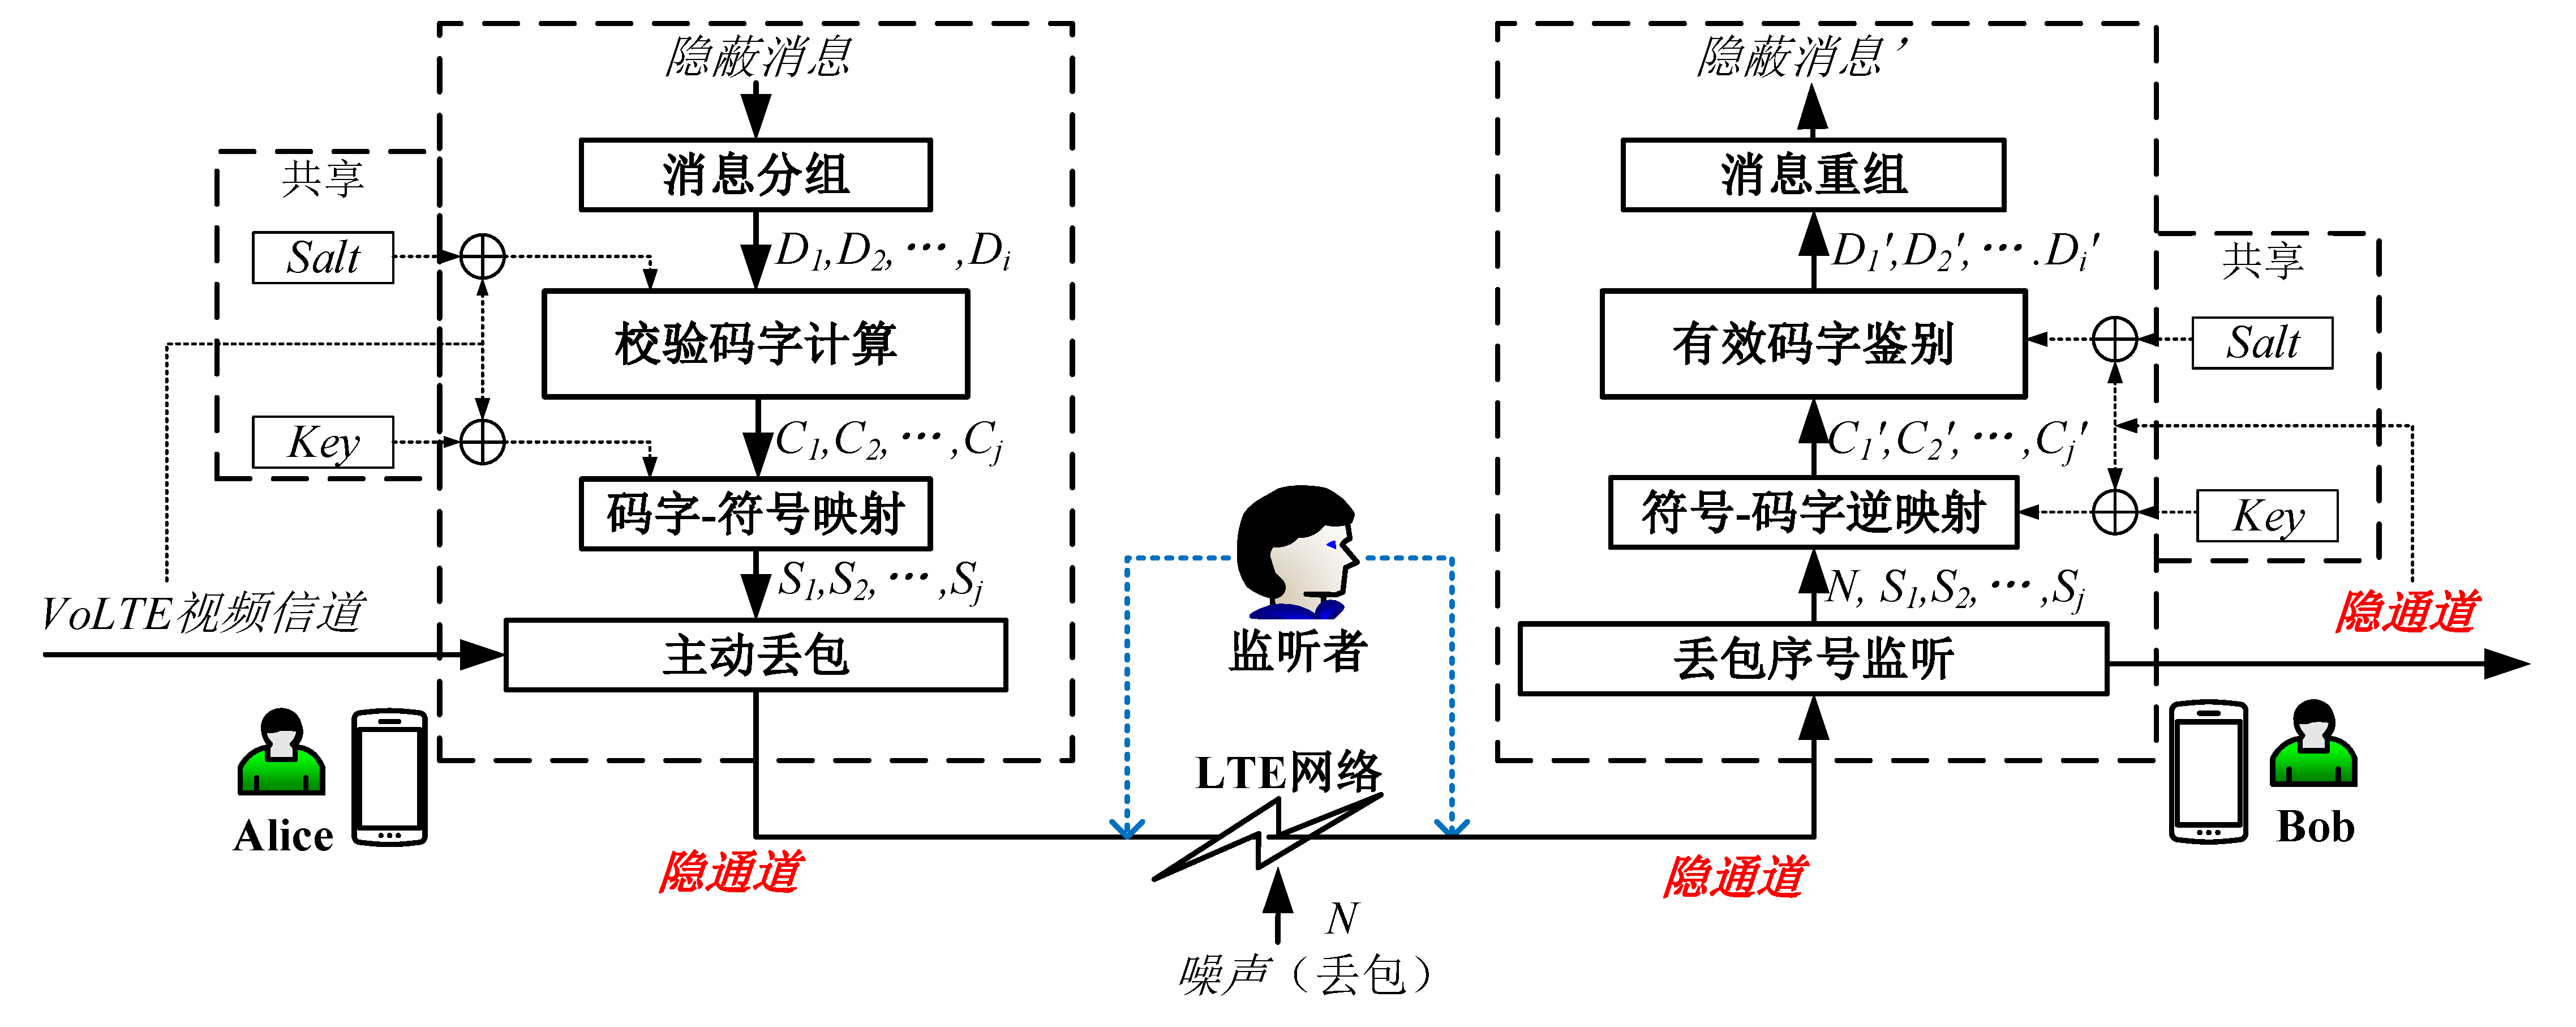
\includegraphics[width=0.98\textwidth]{chapters/chapter4/figures/system-model.pdf}
        \caption{基于Zigzag映射矩阵的时间隐通道系统模型图}
        \label{fig:4:system-model}
	\end{figure}
}

如图\nref{fig:4:system-model},对于用户Alice和Bob,希望通过该时间隐通道传输隐蔽消息,而监听者对两人的所有通信进行了监听,只允许进行被监听的VoLTE通话。在进行传输前,接收方与发送方首先约定一个私有的$Key$及$Salt$,类似消息加密的私有秘钥,用于调制过程中CRC校验生成及映射矩阵初始化。调制过程的消息分组阶段,完成对隐蔽消息的分组,生成定长的消息块$D_{i}$。校验码字计算阶段依赖CRC算法,结合私有$Salt$及宿主信道中提取的随机信息,计算每个码字的校验值,生成所有码字$C_{j}$。码字-符号映射阶段,利用私有$Key$及随机信息初始化映射矩阵,将码字$C_{j}$映射到相对序号$S_{j}$。主动丢包阶段,监控当前的数据包传输状态,并将目标数据包直接丢弃。

VoLTE数据包经LTE网络传输后,时间隐通道与网络噪声叠加。接收方监听到达的RTP数据包序号,并记录下丢失数据包的序号。按照调制过程的逆序,解调过程识别获取的$S_{j}^{'}$,然后参照逆映射矩阵将$S_{j}^{'}$转换为$C_{j}^{'}$,逆映射时映射矩阵的初始化参数与调制阶段保持一致。有效码字鉴别阶段根据CRC校验码字,筛选出符合校验规则的数据块$D_{i}^{'}$。最终消息重组阶段组合所有的消息块,得到隐蔽消息。

\subsection{调制流程}
\label{chap:zigzag:model:modulation}

\insertFigure{
	\begin{figure}[t]
		\centering
        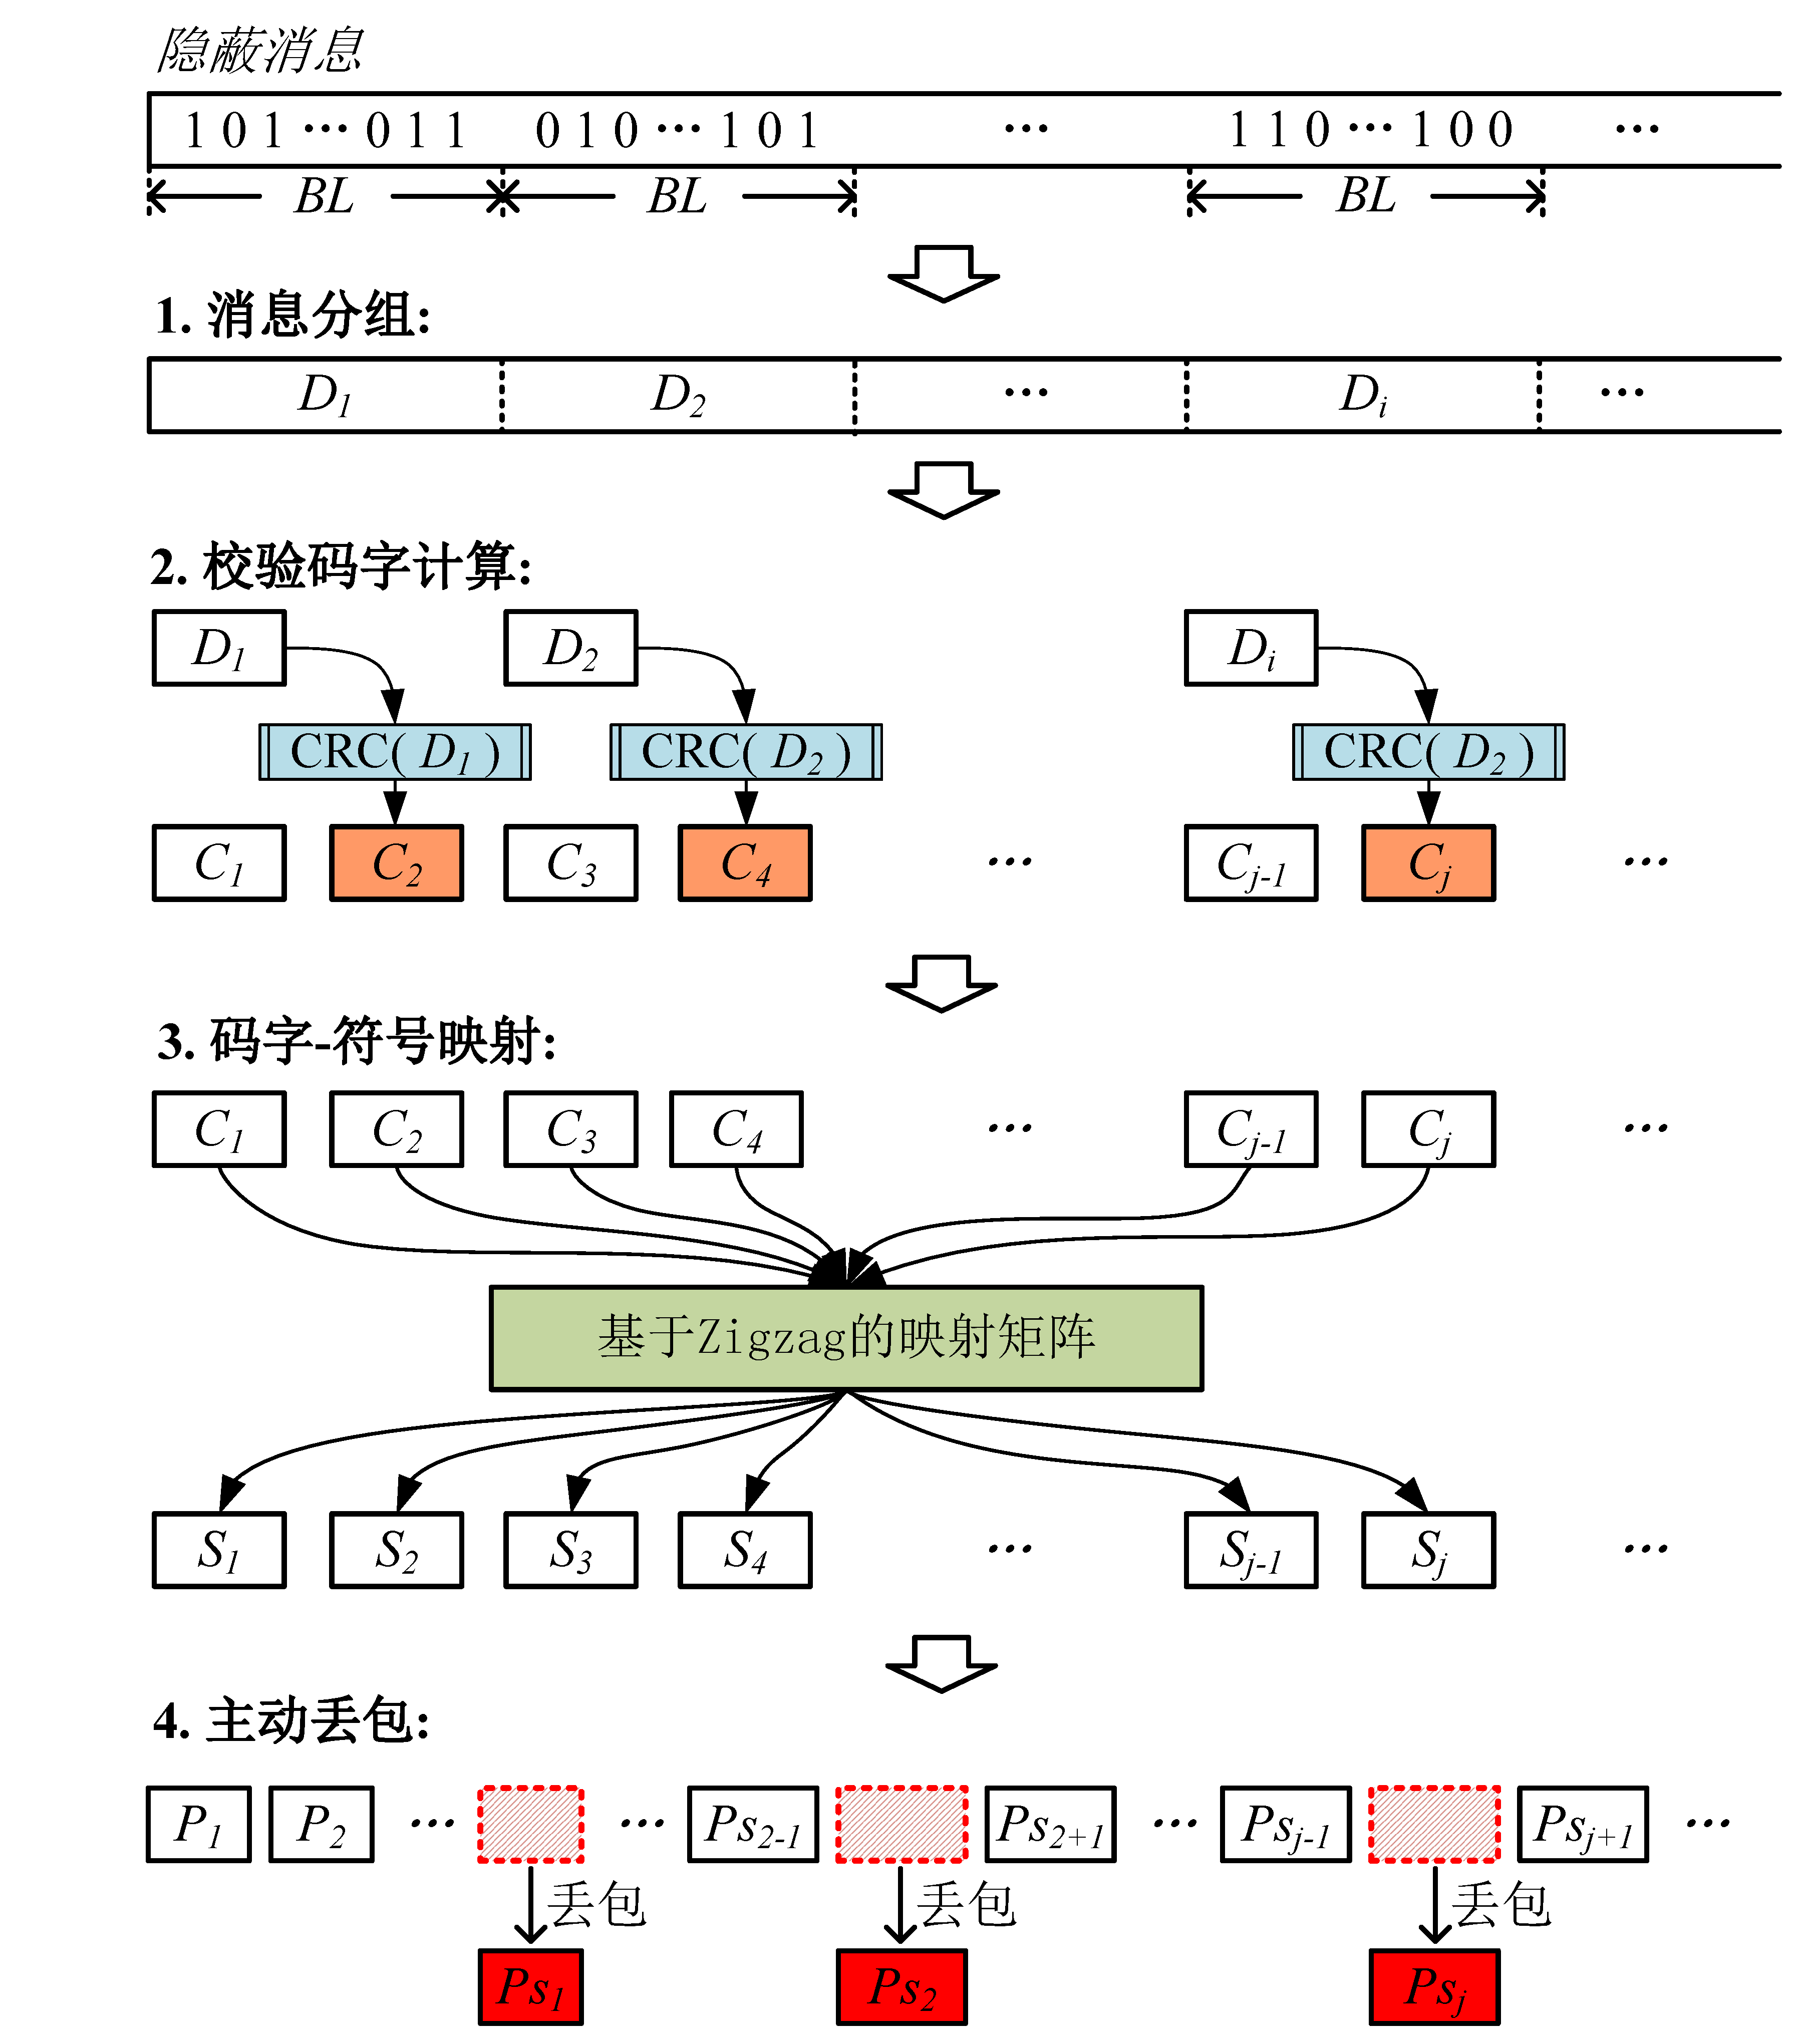
\includegraphics[width=0.85\textwidth]{chapters/chapter4/figures/modulation-flow.pdf}
        \caption{基于Zigzag映射矩阵的时间隐通道调制流程}
        \label{fig:4:modulation-flow}
	\end{figure}
}

如图\nref{fig:4:modulation-flow},调制过程中的处理过程,及数据变化情况可以分为4个阶段,与系统模型中的各阶段对应。要发送的隐蔽消息为输入变量,最终产生的结果是具有序号$S_{j}$的数据包被丢弃。

\subsubsection{分段传输}
\label{chap:zigzag:model:modulation:segment}
隐蔽消息按照参数$BL$,切分为定长的消息块$D_{i}$,每个消息块单独进行调制。通过丢包位置在分段内的相对位置,代表符号$S_{j}$,则传输每个符号需要的数据包数量为$2^{BL}$。在这里,码字内部没有添加额外的校验信息,因此$L_{Codeword}=BL$。

\insertEquation{
    \begin{equation}
    \label{equ:4:throughput}
		Throughput = \frac{L_{Codeword}}{2^{L_{Codeword}}}\times 100(packets/s)= \frac{BL}{2^{BL}}\times 100(packets/s)
    \end{equation}
}

当确定了传输参数$L_{Codeword}$,则该时间隐通道的传输性能可以通过公式(\nref{equ:4:throughput})计算,VoLTE视频数据包传输速率按照统计值$100(packets/s)$计算。在一次通话过程中,发送的数据包总量是有限的,时间隐通道必须提高传输效率。在分段模式下,通信双方不需要同步时钟,便实现通信同步,提高了资源利用率。

\subsubsection{基于CRC的码字校验}
\label{chap:zigzag:model:modulation:crc}

计算CRC校验前,需要结合用户自定义的私有$Salt$,以及由RTP传输流中导出的随机字段。在这里,选择RTP包头中的$SSRC$,与$Salt$进行异或后与消息块$D_{i}$进行拼接,共同作为CRC函数的参数计算摘要结果。计算过程的算法描述如算法\nref{alg:4:codeword-generation},输入参数包括消息及参数信息,最终返回生成的码字序列$C$。

\insertContents{
    \begin{algorithm}[t]
        \renewcommand{\algorithmicrequire}{\textbf{Input:}}
        \renewcommand{\algorithmicensure}{\textbf{Output:}}
        \caption{码字生成}
        \label{alg:4:codeword-generation}
        \begin{algorithmic}[1]
            \REQUIRE $Covert\ Message$,\ $SSRC$,\ $Salt$,\ $L_{Codeword}$
            \ENSURE $C \leftarrow \{\}$
            \STATE $D \leftarrow \{\},\ offset \leftarrow 0$
            \FOR{$offset < length(Covert\ Message)$}
                \STATE $D_{i} \leftarrow Covert\ Message[offset:L_{Codeword}]$
                \STATE append $\ D_{i}\ $ to $\ D$
            \ENDFOR
            \STATE $salt \leftarrow Salt\ \bigoplus\ SSRC$
            \FOR{$D_i\ $ in $\ D$}
                \STATE $C_{j} \leftarrow $CRC16($salt\ //\ D_{i}\ //\ salt$)
                \STATE append $\ D_{i}\ $ to $\ C$
                \STATE append $\ C_{j}\ $ to $\ C$
            \ENDFOR
            \RETURN $C$
        \end{algorithmic}
    \end{algorithm}
}

\subsubsection{映射矩阵}
\label{chap:zigzag:model:modulation:mapping}

映射矩阵实现了码字$C_{j}$到符号$S_{j}$的变换,矩阵中元素的数量由$L_{Codeword}$决定。矩阵的行数与列数如公式(\nref{equ:4:matrix-length}),映射矩阵$\textit{\textbf{M}}$为方阵,且满足$M_{cols}\times M_{rows}=2^{L_{Codeword}}$。映射矩阵的映射关系,是完善本方法保密性的技术之一。图\nref{fig:4:zigzag-matrix}中$M_{1,1}$由1开始,而实际应用中,$M_{1,1}$由用户设定的$Key$及RTP中的随机字段决定,计算公式如公式(\nref{equ:4:matrix-begin})。映射矩阵排布完毕后,对每个元素$M_{i,j}$进行取模,确保最终值$M_{2^{L_{Codeword}-1},2^{L_{Codeword}-1}}$不超过符号范围的上限。

\insertEquation{
    \begin{equation}
    \label{equ:4:matrix-length}
		M_{cols}\ =\ M_{rows}\ =\ 2^{\frac{L_{Codeword}}{2}}
    \end{equation}
    \begin{equation}
    \label{equ:4:mapping}
        S_{j}\ =\ \textit{\textbf{M}}_{C_{j,\ \lbrack L_{Codeword}/2,\ L_{Codeword})},\ C_{j,\ \lbrack 0,\ L_{Codeword}/2)}}
    \end{equation}
    \begin{equation}
    \label{equ:4:matrix-begin}
        M_{1,\ 1}\ =\ (Key\ \bigoplus\ SSRC)\ \%\ 2^{L_{Codeword}}\ +\ 1
    \end{equation}
}

对于码字$C_{j}$,整体长度为$L_{Codeword}$ bit,按照$L_{Codeword}/2$ bit进行划分,可以划分为前半部$C_{j,\ [0,\ L_{Codeword}/2)}$及后半部$C_{j,\ [L_{Codeword}/2,\ L_{Codeword})}$。参照图\nref{fig:4:zigzag-matrix},调制过程中映射矩阵与符号及码字的关系,如公式(\nref{equ:4:mapping})。

\subsection{解调流程}
\label{chap:zigzag:model:demodulation}

\insertFigure{
	\begin{figure}[t]
		\centering
        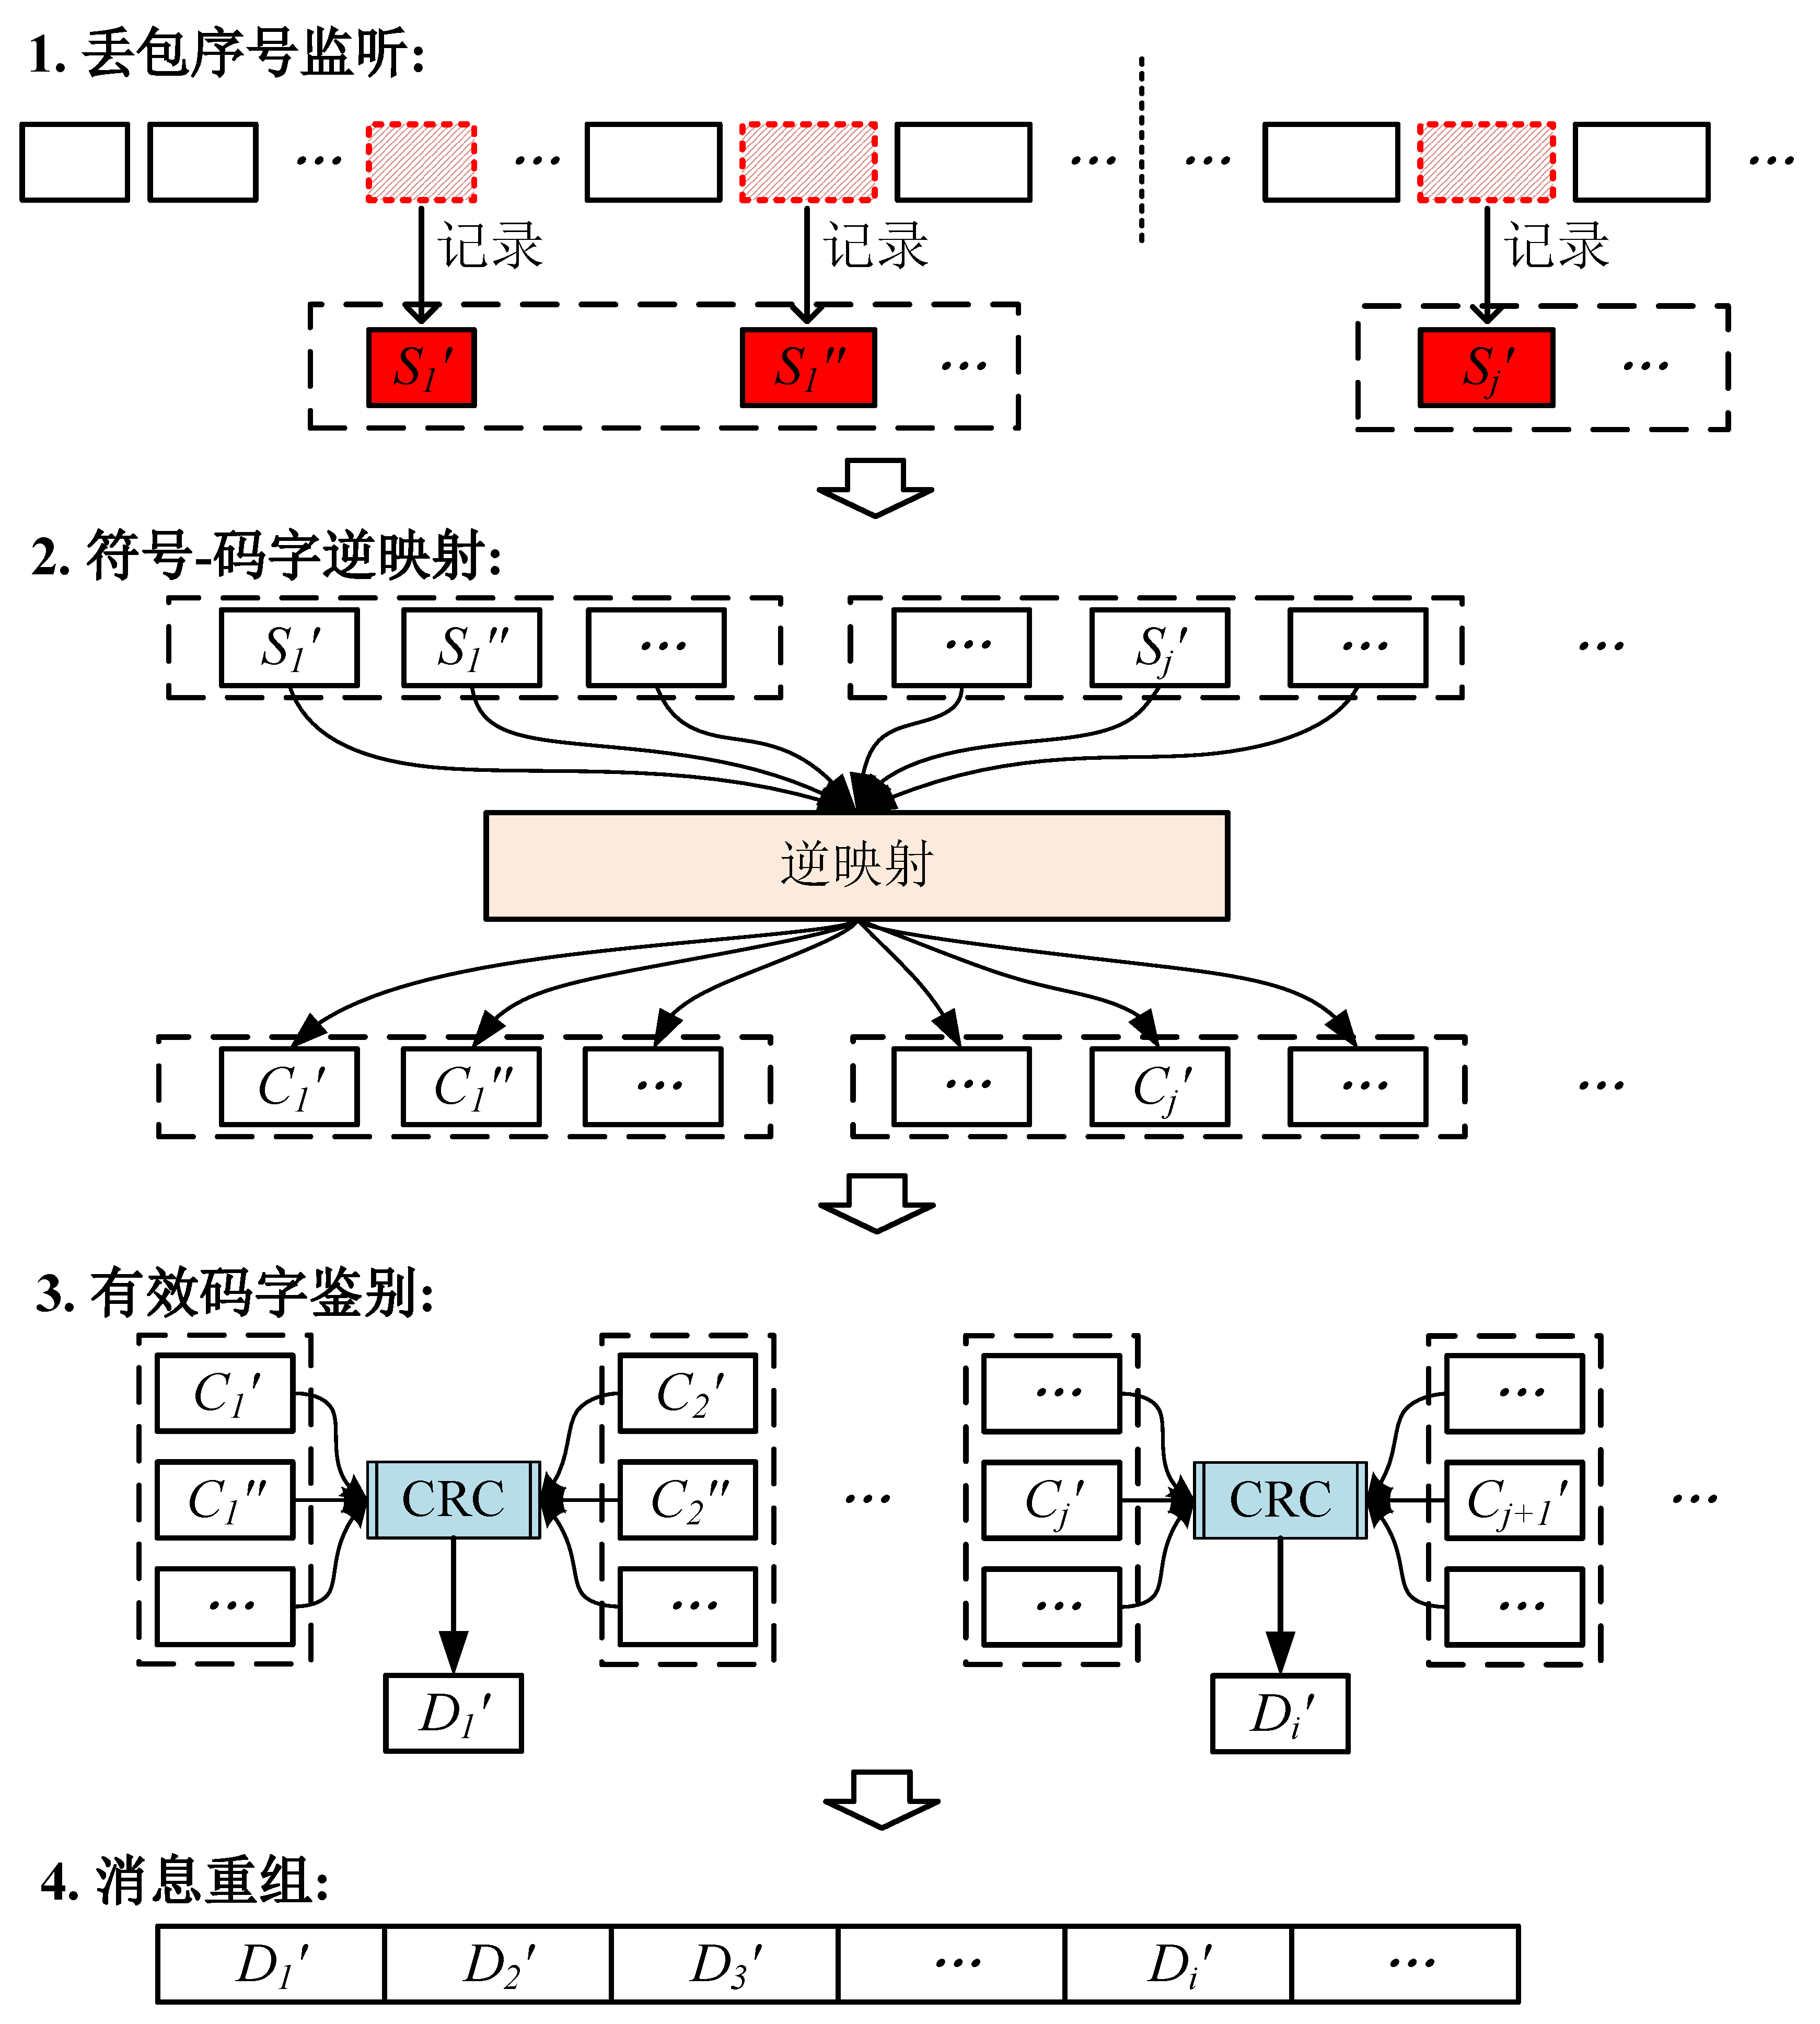
\includegraphics[width=0.85\textwidth]{chapters/chapter4/figures/demodulation-flow.pdf}
        \caption{基于Zigzag映射矩阵的时间隐通道解调流程}
        \label{fig:4:demodulation-flow}
	\end{figure}
}

如图\nref{fig:4:demodulation-flow},解调流程主要分为4各部分,分别为丢包序号监听获取丢包序号、符号-码字逆映射将符号转换为码字、鉴别符合校验规则的码字,以及消息重组得到隐蔽消息。由于网络噪声不可避免,解调过程中每组内存在多个候选的符号或码字,在完成验证前,所有的候选项都视为可能解。

\insertEquation{
    \begin{equation}
    \label{equ:4:group-id}
		j\ =\ \left \lfloor\frac{number\ -\ 1}{2^{L_{Codeword}}}\right \rfloor\ +\ 1
    \end{equation}
    \begin{equation}
    \label{equ:4:symbol}
        S_{j}\ =\ (number\ -\ 1)\ \%\ (2^{L_{Codeword}})\ +\ 1
    \end{equation}
}

根据映射矩阵的规模,每次映射对应的数据包数量为$2^{L_{Codeword}}$,则丢包序号$number$与$j$及$S_{j}$的对应关系如公式(\nref{equ:4:group-id})及公式(\nref{equ:4:symbol})。

\subsubsection{逆映射}
\label{chap:zigzag:model:demodulation:reverse-mapping}

映射矩阵将码字映射为符号,逆映射过程需要按照相同的规则还原码字。对于接收方来说,通过映射矩阵进行逆映射效率较低,需要首先生成映射矩阵的逆映射关系。按照调制过程中\nref{chap:zigzag:model:modulation:mapping}相同的方式,在构建映射矩阵的过程中,创建映射关系$S_{j}\ \rightarrow\ C_{j}$,在添加索引后能够快速完成逆映射。

\insertContents{
    \begin{algorithm}[t]
        \renewcommand{\algorithmicrequire}{\textbf{Input:}}
        \renewcommand{\algorithmicensure}{\textbf{Output:}}
        \caption{有效码字鉴别}
        \label{alg:4:codeword-identification}
        \begin{algorithmic}[1]
            \REQUIRE $\{\{C_{1}',\cdots\},\ \{C_{2}',\cdots\},\cdots\},\ Salt,\ SSRC$
            \ENSURE $D \leftarrow \{\}$
            \STATE $salt \leftarrow Salt\ \bigoplus\ SSRC$
            \FOR{$\{C_{j}',\cdots\},\{C_{j+1}',\cdots\}\ $ in $\ C$}
                \FOR{$C_{j}'\ $ in $\ \{C_{j}',\cdots\}$}
                    \STATE $checksum\ =\ $CRC16($salt\ //\ C_{j}'\ //\ salt$)
                    \IF{$checksum\ $ in $\ \{C_{j+1}',\cdots\}$}
                        \STATE append $\ C_{j}'\ $ to $\ D$
                        \STATE \textbf{break}
                    \ENDIF
                \ENDFOR
            \ENDFOR
            \RETURN $D$
        \end{algorithmic}
    \end{algorithm}
}

\subsubsection{码字鉴别}
\label{chap:zigzag:model:demodulation:identification}

在调制过程中,码字规模$j$是数据块规模$i$的2倍,即$j\ =\ 2\ \times\ i$。因此,解调过程中,可以划分为两部分,分别为奇数组的数据码字及偶数组的校验码字。如图\nref{fig:4:demodulation-flow},鉴别码字的过程中,通过重新计算校验值,判断校验值是否在校验码字中出现,即可判断当前数据码字的有效性。

码字鉴别过程的描述如算法\nref{alg:4:codeword-identification},在计算CRC散列前,首先需要计算附加在数据中的盐值$salt$,同样由用户自定义的盐值$Salt$及随机字段$SSRC$组成。重新计算$C_{j}'$对应的校验码字,如果在$\{C_{j+1}',\cdots\}$中出现,则意味着$C_{j}'$符合校验规则,添加到结果中,进行下一轮辨别。

最终,将得到的所有数据块$D_{i}'$组合,接收方还原出隐蔽消息,解调过程结束。